%====================================================================================================
% Fundamentals
%====================================================================================================
\section{Fundamentals}
This parts goes over the fondamentals of optics necessary to understand futur developpments.
%====================================================================================================
% Seeing
%====================================================================================================
\subsection{Seeing}
\textbf{What's the seeing ?} : \newline In atmospheric optics, the "seeing" refers to the degree of blurring or distortion of astronomical objects
caused by Earth's atmosphere. The Earth's atmosphere is not homogeneous. It has various layers of air with different densities and temperatures.
Theses different layers causes the light passing throught it to be refracted in different ways. This result causes a constantly change of blurring,
distortion and glittering. Especially when looking an object low on the horizon. In our case, at IRSOL, the seeing is 4' of arc. We can go up
to 1' arc in the best case\newline
In general, seeing is determined by the angle of an object seen through the atmosphere, which is affected by factors such as temperature and wind speed.
The result of the seeing measure is the inverse of the "Fried parameter", wich describes the size of the atmospheric cells that cause the blurring.
When the Fried parameter is small, we could say that the seeing have good conditions. That means the image will have minimal blurring and distortion.
While poor seeing conditions have a larger Fried parameter, resulting in significant blurring and distortion of atmospherical objects.
%(Paramètre de Fried => Inverse)
\bigbreak
\textbf{Where are the turbulences} : \newline
First, we need to know how much type of turbulence we could see appearing and where they could be appear.\newline
There are 4 types of turbulence that we could see on the atmosphere. Each type is listed below :
\begin{itemize}
    \item Dome turbulence : \newline Appear when the air as not the same temperature between inside and outside the dome. This turbulence corresponds to
          the mirror turbulence.
    \item Surface trubulence : \newline Appear between the first 10 to 100 meters. Its appearance is due to the cooling by convection of the ground
          heated by the sun. Its minimum is just after the sunrise and its minimum when the sun sets. The evolution of this turbulence is an increasing
          evolution before the zenith and a decreasing evolution after it.\newline
          To counter this turbulence, a site selection is recommanded. For minimize it, the telescope could be place on a tower, away from any surface.
    \item Medium altitude turbulence : \newline Appear between 1.5 to 6 kilometers. Its appearance is due to atmospheric streams and in the thermal
          instabilities of the atmosphere. This turbulence is made up of multitudes of fine turbulent layers of varying densities and of a few hundred
          meters. For minimize it, a measure on the site should be carried out before.
    \item Tropopause and stratospheric turbulence : \newline Could appear between 6 and 20 kilometers. It reach a minimum t 6km and maximum on the
          tropopause between 10 and 20km. Its appearance is due to the strong winds shearing the atmosphere. This tubulence decrease after reach its maximum
          until it disappears after 25 - 30km.
\end{itemize}

%====================================================================================================
% DIMM
%====================================================================================================
\subsection{Differential image motion monitor (DIMM)}
\textbf{What's a DIMM ?} : \newline A differential image motion monitor is an instrument used in atmospheric optics to measure the amount of turbulence
in the Earth's atmosphere. It analyze the movement of stars as their light passes through the atmosphere, wich causes the stars to twinkle and blur.
\newline
The DIMM system consists of mask and split the image in two. After that, each image is recorded with a camera. On each part of this camera, the image
has a different seeing. Theses differences are used to determine the amount of distortion caused by the atmosphere.\newline
If we made a differential measure of theses images, we will get the atmospheric turbulence, wich is expressed as the seeing or the size of the
blurred image of a point source. \newline
The DIMM technique is widely used in astronomical observations, as it provides an objective and quantitative measure of the atmospheric turbulence,
which can affect the resolution and sensitivity of telescopes. It is also used in adaptive optics systems, where it is used to measure the atmospheric
turbulence in real-time, and to correct for the distortions using deformable mirrors.

\bigbreak
\textbf{Structures} : \newline the DIMM system is a relatively simple and robust instrument, which provides an accurate and objective measure of the atmospheric turbulence.
The elements that constitute a Differential Image Motion Monitor (DIMM) are listed below and viewable on the figure
\ref{fig:DIMM_Schematic} :
\begin{enumerate}
    \item Optical path : To create two images of our object, we need something wich will split our object in two. To realize this, a beam splitter could
          should be the best solution. It is also possible to separate the object before it enters the telescope by installing a "mask" before its first
          eyepiece.
    \item Camera : Which records the images of the star. The cameras are usually high-speed, sensitive detectors, such as CCDs or EMCCDs.
    \item Image processing software : The images obtained by the cameras are analyzed by software that measures the distortion caused by the atmosphere.
          The software calculates the difference in the distortion measurements obtained by the two telescopes, which allows for the determination of the
          atmospheric turbulence.
    \item Control and data acquisition system : The DIMM system is usually controlled by a computer, which also acquires and stores the data obtained by
          the cameras. The data can then be used to calculate the atmospheric turbulence, and to analyze the seeing conditions.
\end{enumerate}
\begin{figure}[H]
    \centering
    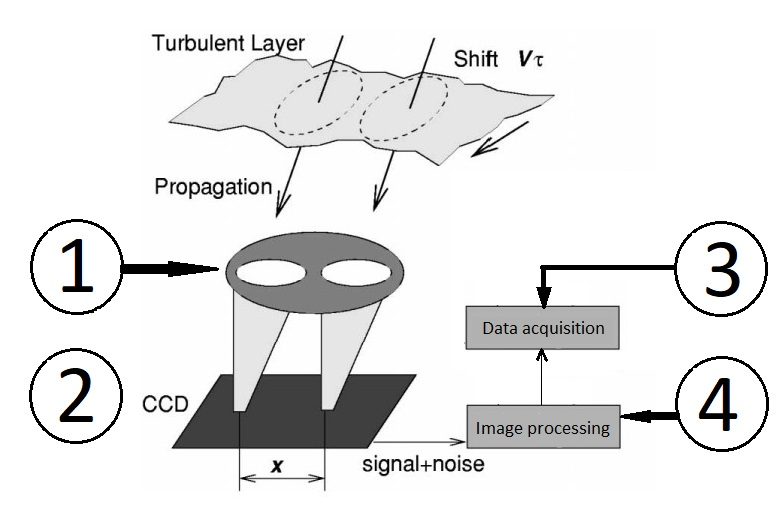
\includegraphics{assets/figures/Theory/DIMM_Schematic.jpg}
    \caption{Schematic principe of DIMM}
    \label{fig:DIMM_Schematic}
\end{figure}

%====================================================================================================
% Equation
%====================================================================================================
\section{Usual mathematical functions}
The basic mathematical functions used and quoted in the theoretical part are found in this section.
\subsection{Nyquist frequency}
\begin{equation}\label{eq:Nyquist}
      n_1*\sin(\theta_1)=n_2*\sin(\theta_2)
\end{equation}
\subsection{Refraction with Snell-Descartes}
\begin{equation}\label{eq:Snell}
      n_1*\sin(\theta_1)=n_2*\sin(\theta_2)
\end{equation}
\subsection{Trigonometry}
\begin{equation}\label{eq:Trigo_sin}
      sin(\alpha) = \frac{opposite}{Hypotenuse}
\end{equation}
\begin{equation}\label{eq:Trigo_cos}
      cos(\alpha) = \frac{Adjacent}{Hypotenuse}
\end{equation}
\begin{equation}\label{eq:Trigo_tan}
      tan(\alpha) = \frac{opposite}{Adjacent}
\end{equation}
\subsection{Equation of the affine line}
\begin{equation}\label{eq:DoiteAffine}
      Y = a*X+b
\end{equation}
